\documentclass[10pt]{standalone}

\usepackage{pgfplots}
\usetikzlibrary{calc, tikzmark, shapes, shapes.arrows, arrows, 3d, positioning}
\pgfplotsset{compat=1.17}

\begin{document}
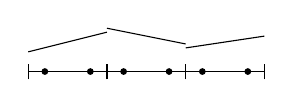
\begin{tikzpicture}
	\draw (0,-.1) grid (3,.1); 
	\foreach \x in {0,1,2}{
		\filldraw[black] (\x + 0.21132487,0) circle[radius=1pt]; 
		\filldraw[black] (\x + 0.78867513,0) circle[radius=1pt]; 
	}

	\draw[domain=0:1, smooth, variable=\x, black] plot ( \x, .25 + \x*.25); 
	\draw[domain=1:2, smooth, variable=\x, black] plot ( \x, .75 -\x*.2);
	\draw[domain=2:3, smooth, variable=\x, black] plot ( \x, .15*\x);  
\end{tikzpicture}
\end{document}